\chapter{Rotating solar systems and radio astronomy}

\section{Introduction} 
You might think that being limited to radio signals, the kinds of observations you could make and the information you could gather would be relatively small. In fact, there are a wide range of observations and interesting phenomena which can be detected using a radio telescope. From the elemental make up of a distant planet's atmosphere, to the detection of extreme astronomical objects. In fact, we can use observations of signals from hydrogen clouds in the galactic plane and, using the knowledge we gained of the Doppler shift, obtain an estimate for the distribution of matter in the Milky Way. By now you know how to use radio signals to find velocity, but how do you use velocity to find mass? In this lab, not only will you learn how we can estimate the mass distribution of an orbital system, but you will also learn the basics of using the Small Radio Telescope, which lives on the roof of Kersten Physics Teaching Center.

\section{Learning Goals}
\begin{itemize}
	\item Make predictions about large, gravitationally bound systems based on observations of smaller scale systems.
	
	\item Make observations using the Small Radio Telescope (SRT) and interpret the data
	
	\item Calibrate the SRT and understand the uncertainty by measuring background noise in the Chicago sky 
\end{itemize}

\section{Team roles}

\textbf{Decide on roles} for each group member. The available roles are:

\begin{itemize}
	\item Facilitator: ensures time and group focus are efficiently used
	\item Scribe: ensures work is recorded
	\item Technician: oversees apparatus assembly, usage
	\item Skeptic: ensures group is questioning itself
\end{itemize}

These roles can rotate each lab, and you will report at the end of the lab report on how it went for each role. If you have fewer than 4 people in your group, then some members will be holding more than one role. For example, you could have the skeptic double with another role. Consider taking on a role you are less comfortable with, to gain experience and more comfort in that role.

Additionally, if you are finding the lab roles more restrictive than helpful, you can decide to co-hold some or all roles, or think of them more like functions that every team needs to carry out, and then reflecting on how the team executed each function.

\section{Masses and Orbital Velocity} %working title only
One of the main labs you will carry out this quarter is a measurement of the motion of the Milky Way using the SRT. It is important that when you make these measurements that you understand the results you obtain. In this experiment, you will learn how the specific observations you will make can be used to make some predictions about the Milky Way. 

\subsection{Goal}
Learn how new phenomena can be predicted or inferred from basic physical principles and how to interpret rotation curves. 

\subsection{Equipment}

\begin{itemize}
	\item Desmos Graphing Calculator: \url{https://www.desmos.com/calculator}
\end{itemize}

\subsection{Steps}

\begin{steps}
	\item First, we know from Newton's first law that the force on an object is equal to its mass times its acceleration, $F=ma$. We also know that an object moving in a circle will experience an acceleration towards the center of its path which is given by $a = \dfrac{v^2}{r}$, where $v$ is the velocity of the object and $r$ is the radius the circle it travels along. Combine these two equations to find an equation for the force experienced by an object undergoing circular motion. \textbf{Record your derivation and final equation.}
	
	\item Objects in orbit also move in an approximately circular path and the force of gravity they experience is given by $F = G\dfrac{Mm}{r^2}$, where $M$ and $m$ are the masses of the two objects and $G$ is the gravitational constant. Using the equation you found in the previous step, derive an equation for the velocity of the orbiting object as a function of its radius.\textit{Hint: plug equations into each other to remove variables that are common in both equations. Your final equation should be in terms of $v$, $M$, $r$, and $G$}. \textbf{Record your derivation and final equation.}
	
	\item Create a plot of your equation for the velocity as a function of radius, for example using the online graphing calculator listed in the equipment. To plot it, type the equation in the left side of the screen. It will graph $y$ on the vertical, $x$ on the horizontal axis, so use $y$ in place of your $v$ and $x$ in place of your $r$. For the variables $M$ and $G$, click the ``add slider'' button so you can plot the shape of the curve. You can leave them set to equal 1, since we are using this to see the shape of the curve, not the absolute value. \textbf{Include this graph in your report.}

	\item Adjust the mass slider to larger values and observe what happens to the curve. How does it change? \textbf{Record your answer.}
\end{steps}

The graph you created is called a \textit{rotation curve}, which plots the orbital velocities of objects in an orbital system against their distance from the center. Using these curves, it is possible to learn a lot about the system it describes.

When you first derived the equation for rotational velocity, you assumed that $M$ represented the mass for a single object at the center. Now we will assume that this equation holds true in the case that $M$ represents the total mass contained within the orbital radius. This assumption is valid for a spherically symmetric system, which is a good enough approximation for us. Let's explore some cases for different mass distributions.

\begin{steps}
	
	\item For the case where the mass is uniformly distributed in a disk, the total enclosed mass increases as $r^2$. To graph this, delete the $M$ slider and create a new expression $M = c x^2$. How is this curve different from the previous one? \textbf{Include your answer and plot in your report.}
	
	\item Play with different mass distributions by changing the equation for $M$ and observing how the curve changes.
	
	\item The rotation curve for a sample orbital system is shown in Figure \ref{sbr:fig:solar-rot}. Change the mass formula in your plot to visually match the shape of this curve. How is the mass distributed in this orbital system? \textbf{Record your plot, mass equation, and answer.}
	
	\item Another rotation curve is shown in Figure \ref{sbr:fig:rotations-a-b} (line B). Change the mass formula in your plot to visually match the shape of this curve, especially the curve at medium and long distances. How is the mass distributed in this orbital system? \textbf{Record your plot, mass equation, and answer.}
\end{steps}

\begin{figure}
	\centering
	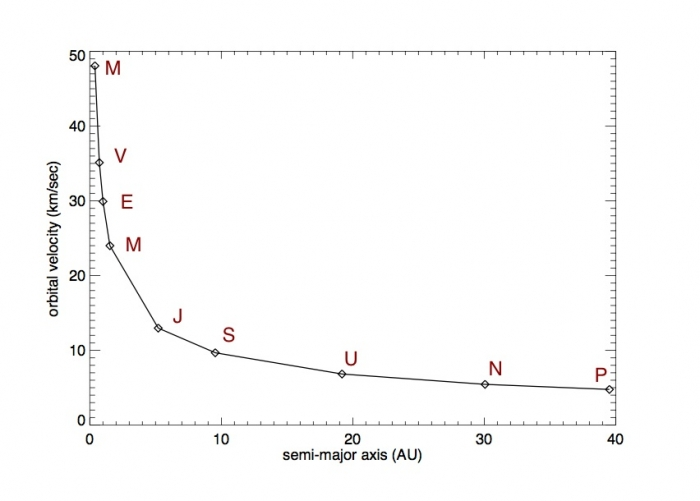
\includegraphics[scale = .6]{srt-background-rotation/keplerian-orbit.jpg}
	\caption{Rotation curve of an example orbital system, where each of the objects marked on the graph are orbiting the center of the system.}\label{sbr:fig:solar-rot}
\end{figure}

\begin{figure}
	\centering
	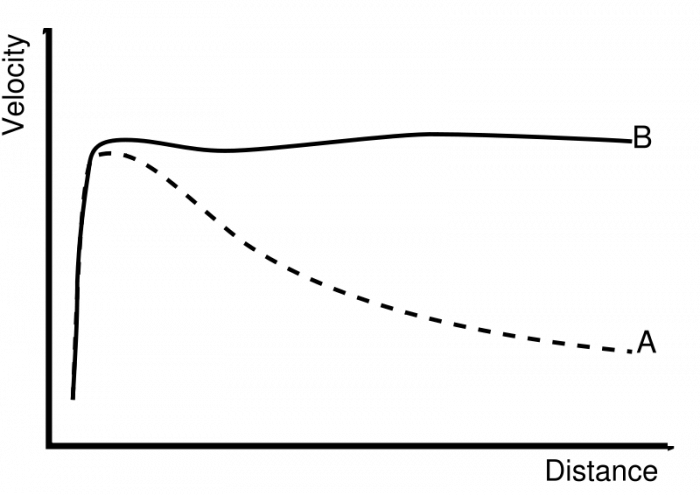
\includegraphics[scale = .3]{srt-background-rotation/galactic_rotation_curve}
	\caption{Rotation curves for two example orbital systems A and B.}\label{sbr:fig:rotations-a-b}
\end{figure}

\begin{steps}
	\item Look up information on the masses of the planets in the solar system as well as the Sun. Which of the rotation curves would you expect the solar system to have? \textit{It might help to add up all the masses and see how much each planet contributes to the total mass.} \textbf{Record your answer.}
\end{steps}

\section{How uniform is the sky in Hyde Park?} %working title only

While learning about the theory behind making astronomical observations can be useful, the best way to gain an intuition for these concepts is through hands on experience. For this experiment, you will learn how to operate the small radio telescope located on top of the Kersten Physics Teaching Center.

Given that there are background sources that can interfere with our
measurements of real sky signal, before we proceed to make any measurements,
it is instructive to explore just how uniform the sky is in Hyde Park.

\subsection{Background noise}

The telescope is sensitive to all sources on the sky, as well as buildings, etc.
Although the telescope is most sensitive over a small area of sky it does have
some low sensitivity to sources at much larger angles from its pointing position.
Radio power generated by cell phone towers and wireless devices within
buildings can cause significant addition signals even though the 1420 MHz band
that we are using is protected for radio astronomy by law against such
interference. Communication devices operate near our frequency and do not
always suppress power in our frequency bands; although the fraction of the radio
power in these sidebands is tiny, our telescope is very sensitive and we can
detect this interference. Human-caused interference can be distinguished from
astronomical sources because it is usually fixed in position while astronomical
sources move across the sky.



\subsection{Telescope Control}
Unfortunately, you will not be able to directly control the telescope and it will instead be controlled by a designated telescope technician. However, you should still learn the basics of controlling the telescope so you can give the technician proper observation instructions. In this case, the technician will act as your hands when operating the telescope, inputting the commands you give them.

\begin{figure}
	\centering
	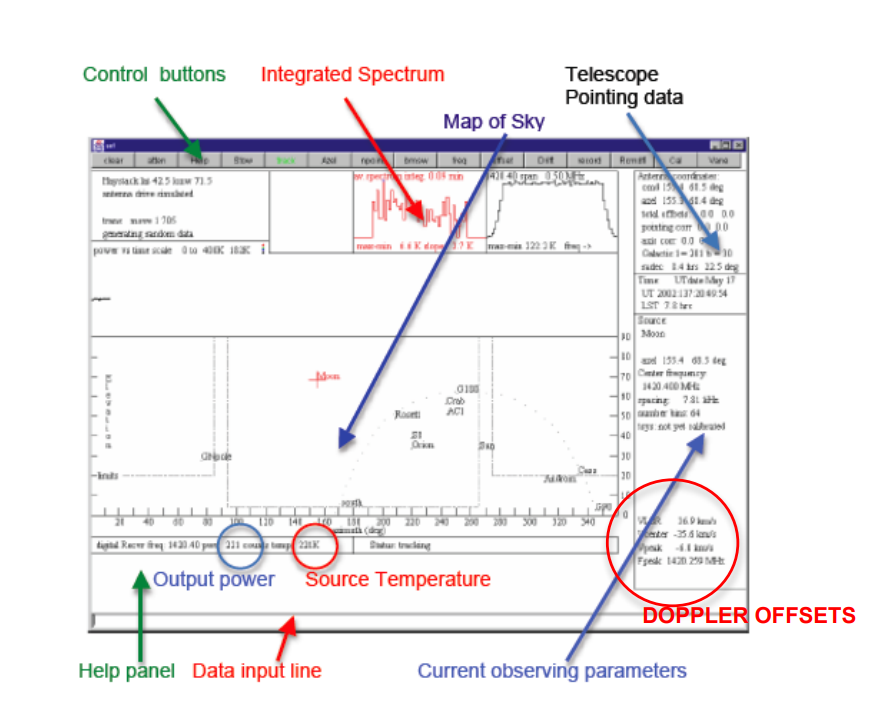
\includegraphics[scale = .9]{srt-background-rotation/display_diagram}
	\caption{Screenshot of SRT control interface with various information labeled.}\label{sbr:fig:srt-display}
\end{figure}

\subsection{Control Buttons}
The control panel display, shown in Figure \ref{sbr:fig:srt-display}, has a line of control buttons at the top that set
up a command for the telescope. For instance, if you want to change the receiver
frequency, you click on the “freq” button. Instructions and help information are
then displayed in the help panel below the map while the cursor is pointed to the
button (This field is blank when you move the cursor away). If you want to
change the frequency, then type data into the data line (e.g. “1420.4 4”), click
“enter” or “return”. Be sure you leave a space between 1420.4 (which is the
frequency) and the number 4 (which sets the bandwidth of the system). The
current observing parameters will be updated in the appropriate box.

\subsection{Control Display \& Sky Map}
The control panel shows a map of the current sky in Azimuth and
Elevation units. 0 degrees azimuth points North, 90 degrees points East, 180
degrees points South and 270 degrees points West. The horizon is at 0 degrees
elevation and Zenith is at 90 degrees. The telescope can point to about 85
degrees in elevation.
The map displays objects visible at the current time. The software tracks
an object or a given azimuth and altitude position, including corrections for the
rotation of the earth. Also displayed on the map are various individual
astronomical sources and a track of dots that show the plane of the Milky Way.
The Longitude of points along the equator of the Milky Way are shown as Gxxx,
where xxx is the Galactic longitude. We have an unobstructed view of all objects
above about 20 degrees.

\subsection{Pointing the Telescope}
You can point to any given position in the sky by clicking on the “AzEl”
button and then typing the desired Azimuth and Elevation in the command line at
the bottom of the display. (e.g., 30 45 “enter” will send the telescope to a position
of 30 degrees azimuth and 45 degrees elevation). When you enter a position you
will see a yellow cross and the CMD numbers will change to these numbers. 

When “track” shows up in green at the top of the display, the telescope has
acquired the position and is tracking it, this holds for sources. If the telescope
does not move, then you probably have to click on “track”.
Occasionally the telescope motor will get stuck and stall. Normally it fixes
itself automatically by going back to the “Stow” position (where it is stowed after
every observation), but if it remains stalled for several minutes click “Stow” to do
so manually. This can be a nuisance and time-consuming but you should still be
able to obtain the necessary data if this happens.

\subsection{Temperature and Calibration} 

In radio astronomy, it is usual to interpret the measured antenna signal in
terms of temperature, as if the measured source is a blackbody, and fills the full
field of view of the telescope. This isn’t necessarily the case, but it’s often a good
approximation and gives a physical parameterization of the measured power. This is why the telescope outputs a temperature. This is not that the SRT is actually measuring the object's temperature, rather, it is simply interpreting the power it receives as a temperature. Since the telescope itself has a temperature, we must perform a calibration step to have it account for it.Similarly, when calibrating, the telescope will display a system temperature $T_sys$ which interferes with our measurements. When calibrating, we account for $T_sys$ and it is subtracted from our measurements. 

\begin{framed}
As a class, you will work together to collect all the necessary data. Each group will collect 2--3 points of data, and then you will share the data among the class.
\end{framed}

\subsection{Calibration Steps}
\begin{steps}
	\item Set the receiver frequency to 1416MHz by clicking on the Freq button, typing “1416 1” in the	command line, and pressing Enter. At this frequency, you will detect the continuum radiation. That is, radiation emitted relatively uniformly over a broad band of frequencies.

	\item Click on the AzEl button and type an Az and El for a blank part of the sky
	(e.g., azimuth and elevation: 10 35; check on the display to make sure you
	select coordinates away from the Galactic plane and from the Sun) into
	the data input line at the bottom of the control panel and then
	hit “enter”. You should see the telescope start to
	move in elevation. The telescope position is printed out in the top right
	panel of the control display. The top line gives the command position
	(which should reflect the position you typed in for AzEl) and the next line
	gives the actual position.
	
	\item When the telescope position is settled (i.e., the cross on the sky display is
	red and the “Track” button at the top of the display is green), click “Clear”
	and write down the raw output power and temperature. Click
	on Cal button and watch these numbers. The system will record the output
	power itself and then switch on the noise source. The computer will then
	calculate the temperature of the sky at that point, which includes the
	system noise temperature. \textit{Note that you should “Clear” before each new
	observation, for both calibration and data, since the telescope is
	continually integrating and thus keeps all the previous data since it was
	last cleared.}
	
	\item Repeat the calibration a few times until you read a stable system temperature $T_{sys}$. Wait around 1 minute between calibrations.
\end{steps}

\subsection{Measuring the noise}

\begin{steps}
	\item Make sure the frequency is set to 1416 MHz by clicking on freq and typing
	in 1416 1
	
	\item From the telescope pointing that you used in the previous exercise (say
	[az,el]=[10,35]) point the telescope 15 degrees lower in elevation (at the
	same azimuth) and 20, and 40 degrees higher in elevation. Repeat the
	calibration at each of these positions 2--3 times and record azimuth and
	elevation of the pointings and values of the sky temperature and system
	temperature displayed by the SRT console. Avoid labeled astronomical
	objects.

	\item After you are done with measurements at different elevation, return to your
	original elevation and change azimuth with step of 50 or 75 degrees (at
	constant elevation) and repeat calibrations 2--3 times at each pointing.
	Record azimuth and elevation of the pointings and values of the sky
	temperature and system temperature displayed by the SRT console.
	
	\item How uniform is the radio sky around Hyde Park? In your lab report,
	discuss the uniformity of the sky signal and system temperature based on
	your measurements. Include a table of your measurements and your
	interpretation and conclusions.
\end{steps}

\section{Report checklist}

Include the following in your lab report. See Appendix~\ref{cha:lab-report-format} for formatting details. Each item below is worth 10 points.

\begin{enumerate}
	\item Derivation of $v(r)$ equation with plot and description of how curve changes (Steps 1--4)
	\item Answer and graph of rotation curve with uniform disk (Step 5)
	\item Graph, mass equation, and answers for two rotation curves (Steps 7--8)
	\item Predicted rotation curve for the Solar System (Step 9)
	\item Calibration raw output power, temperature, and final system temperature (Steps 12--13)
	\item Table of azimuth, elevation, sky temperature, and system temperature (with time and date of each observation), with your group's observations identified (Steps 15--17)
	\item Discussion of sky uniformity with conclusions (Step 17)
	\item A 100--200 word reflection on group dynamics and feedback on the lab manual. Address the following topics: who did what in the lab, how did you work together, how group roles functioned, what successes and challenges in group functioning did you have, and what would you keep and change about the lab write-up?
\end{enumerate}